%************************************************
\chapter{Multifidelity Bayesian Optimization for Accelerated Feedback Controller Tuning}\label{ch:mfbo} 
%************************************************

\section{Introduction}
\label{sec:intro}
Laboratory unit operations such as reactors and distillation columns  are often subjected to many processes in short window of time. For each new process, the control systems of these unit operations need to be re-tuned, which can be a time and labor intensive endeavor. As an example, in the distillation laboratories at BASF, operators often spend days attempting to find the best tuning parameters for a new distillation column setup, which is unacceptable given the short timelines of operating a testing laboratory. While it is possible to use model predictive control, decentralized PID controllers are often used due to their robustness and simplicity. In this work, we aim to develop a fast method tuning controllers and apply this method laboratory distillation columns.

There are a wide variety of existing tuning protocols ranging from heuristics such as Ziegler Nichols \citep{Ziegler1942} and its refinements \citep{Hang1991} to tuning using analytical equations from models via methods such as  Internal Model Control \citep{Copeland2010}. However, extending these to multi-input multi-output systems has been challenging, often requiring additional optimizations \citep{Nandong2013, Nandong2015}. Optimization-based methods have shown promise \citep{Pajares2019, Sumana2010, Rajapandiyan2012, Behroozsarand2012}, but these methods have been difficult to apply in practice due to the large number of iterations they require. Recently, Bayesian optimization, a technique for optimizing expensive to evaluate functions, has shown promise for tuning controllers \citep{NeumannBrosig2020, Fiducioso2019, Khosravi2020, Konig2020, Fujimoto2022, Brunzema2022, Khosravi2022}, but this method still often requires tens to hundreds of iterations, making it too materially expensive for laboratory chemical processes. 

In this work, we introduce a novel optimization approach that combines simulation and Bayesian optimization (BO) to effectively tune controllers. Specifically, we develop a dynamic simulation of a distillation column that is only a low fidelity approximation of the original distillation simulation. We then develop a Bayesian optimizaiton algorithm can use these simulations, despite their low fidelity, to reduce the number of iterations required to find optimal controller parameters. 

\begin{figure}
    \centering
    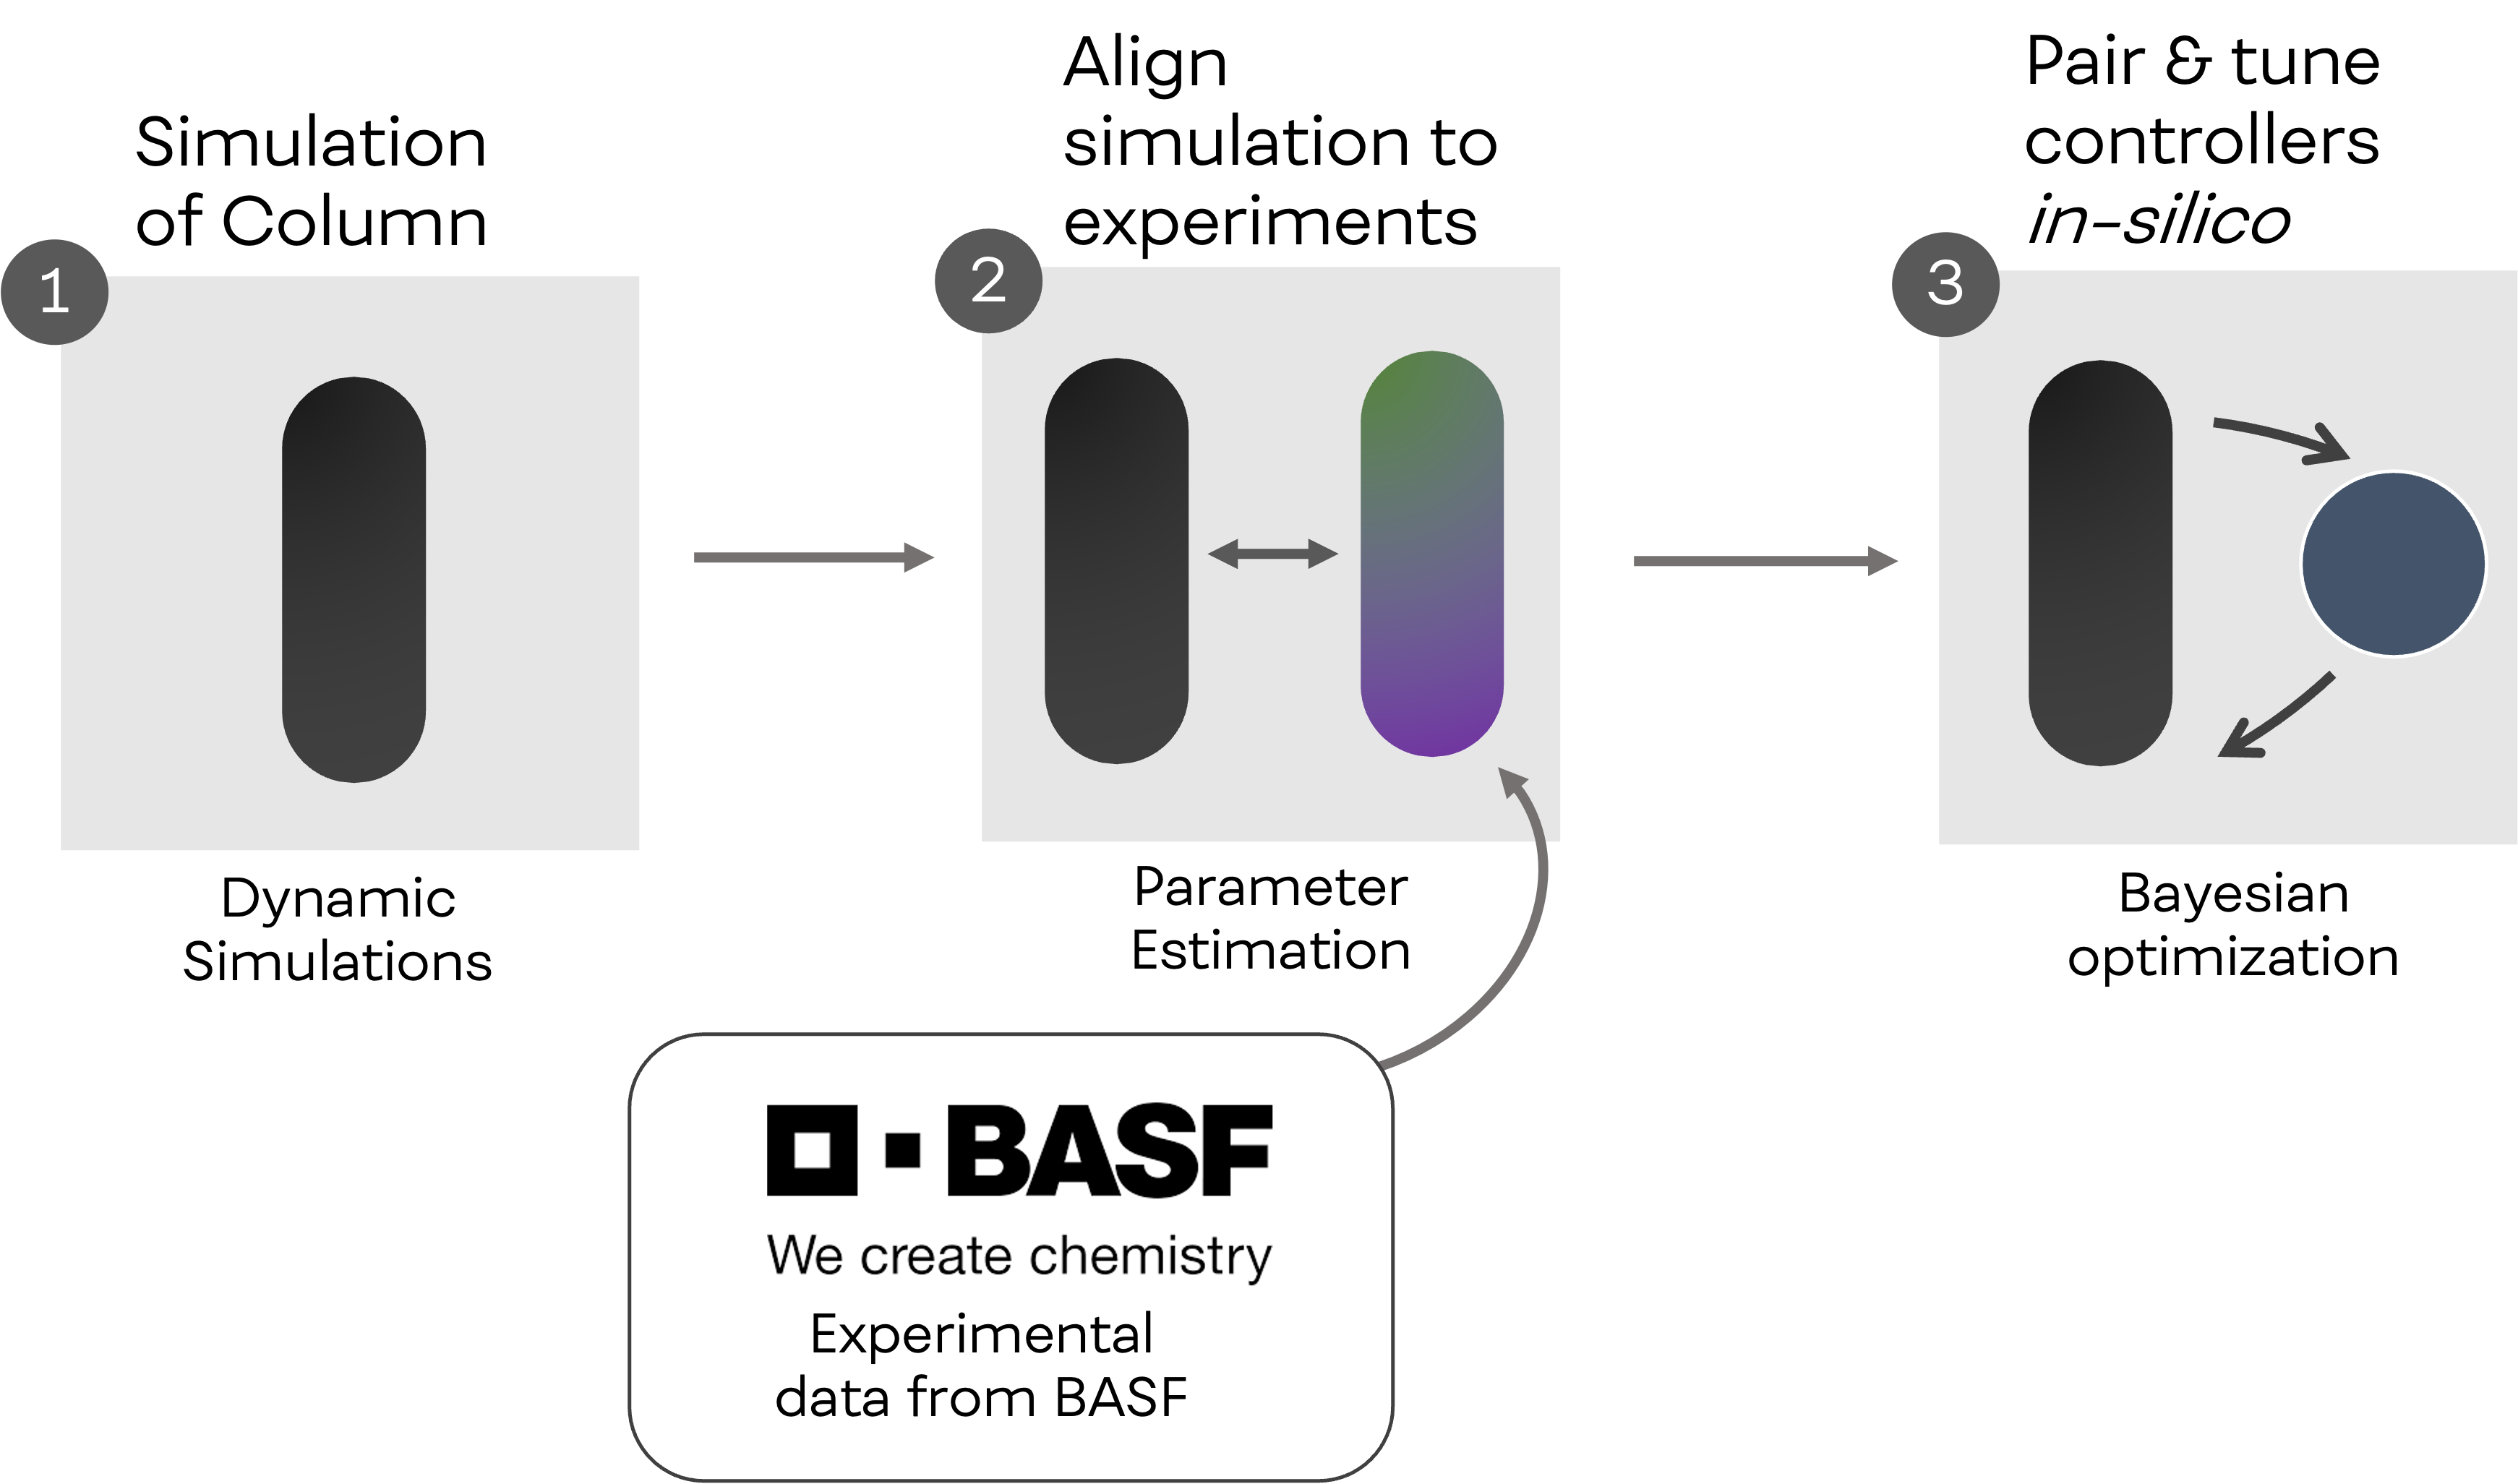
\includegraphics[width=0.8\textwidth]{gfx/Chapter06/tuning_workflow.png}
    \caption{Three step workflow for distillation controller design and tuning. }
    \label{fig:tuning_workflow}
\end{figure}

\section{Methods}

\subsection{Controller Tuning as an Optimization Problem}

Tuning involves identifying the three parameters of the PID equation, $K^P$, $\tau_I$ and $\tau_D$:

\begin{equation}
    \label{eq:PID_defining_equation}
    u(t) = K^P e(t) + \frac{1}{\tau_I}\int_0^t e(t')dt' + \tau_D \frac{de(t)}{dt}
\end{equation}
where $u(t)$ is the controller output that is feed into the actuator (e.g., a valve) and $e(t)$ is the error at time $t$

We formulate the problem of controller design and tuning as an optimization problem. The aim is to find a set of controller pairings and tunings that will achieve desired behavior. We define good controller behavior as minimizing the integral absolute error (IAE) for each controlled variable and minimizing total controller movement (CM):
\begin{equation}
    \min_{\Omega}(IAE_1, IAE_2, IAE_3, CM_1, CM_2, CM_3)
\end{equation}

\begin{equation}
    IAE = \int_0^T \vert y_{sp}(t) - \hat y(t) \vert dt
\end{equation}

\begin{equation}
    CM = \sum_{t=1}^{T}( \vert x_t - x_{t-1} \vert)
\end{equation}
where $y_{sp}$ is the setpoint,  $\hat y$  is the value of  the variable, T is the time horizon. 

\subsection{Multi-Objective and Multifidelity Bayesian Optimization for Controller Tuning}

We solved the controller tuning problem using multi-objective Bayesian optimization problem. We trained an independent GP to predict each controller objective (IAE, CM) given the relevant controller parameters.   Since our problem is multi-objective, we used a multi-objective acquisition function, namely the q Noisy Expected Hypervolume Improvement (qNEHVI). This acquisition function has a balance of computational efficiency and fidelity resulting in an ability to find the pareto front of trade-offs between objectives quickly. 

We also desired to see if simulations could accelerate controller tuning. We developed a differential equation simulation of a distillation column that was aligned to experimental data using both steady state and dynamic parameter estimation (see Supplementary Material for full details). To leverage the simulation, we used a multi-task GP that could be trained on both the less abundant high fidelity experimental data and the more abundant low fidelity simulation data. We hoped that the multi-task GP could learn the correlation between the simulation and the experimental data and thus make better predictions on the experiments with less data.

In practice, we optimized the high fidelity task when selecting  a new set of controller parameters ton run an experiment in the laboratory. Then, while waiting for the laboratory results, we used optimize the lower fidelity task using the differential equation simulation with the most recently estimated parameters. 


\subsection{Distillation Simulation}\label{sec:distillation_model}

In order to base our simulations in reality, we collected experimental data for separation of a 50/50 methanol-water mixture at the laboratories of BASF SE in a 80 tray column with one bubble cap on each stage. The column was kept at approximately 800 mbar vacuum, and a Julabo evaporator was used as the reobiler. The column occupies approximately three stories in the BASF lab.  Three days of data were collected, one of which is used for parameter estimation and the rest for validation. 

Our goal in simulating a distillation columns was to find a balance between model complexity and accuracy. We opted for a formulation similar to \citet{Diehl2001}, which assumes constant pressure drop over time but includes the MESH equations and hydrodynamics. As shown in Figure \ref{fig:column}, $N$ is the number of trays in the distillation column. The distillation column is numbered from the bottom, starting with the reboiler as $i=0$ and condenser as $i=N+1$.  

\begin{figure}
    \centering
    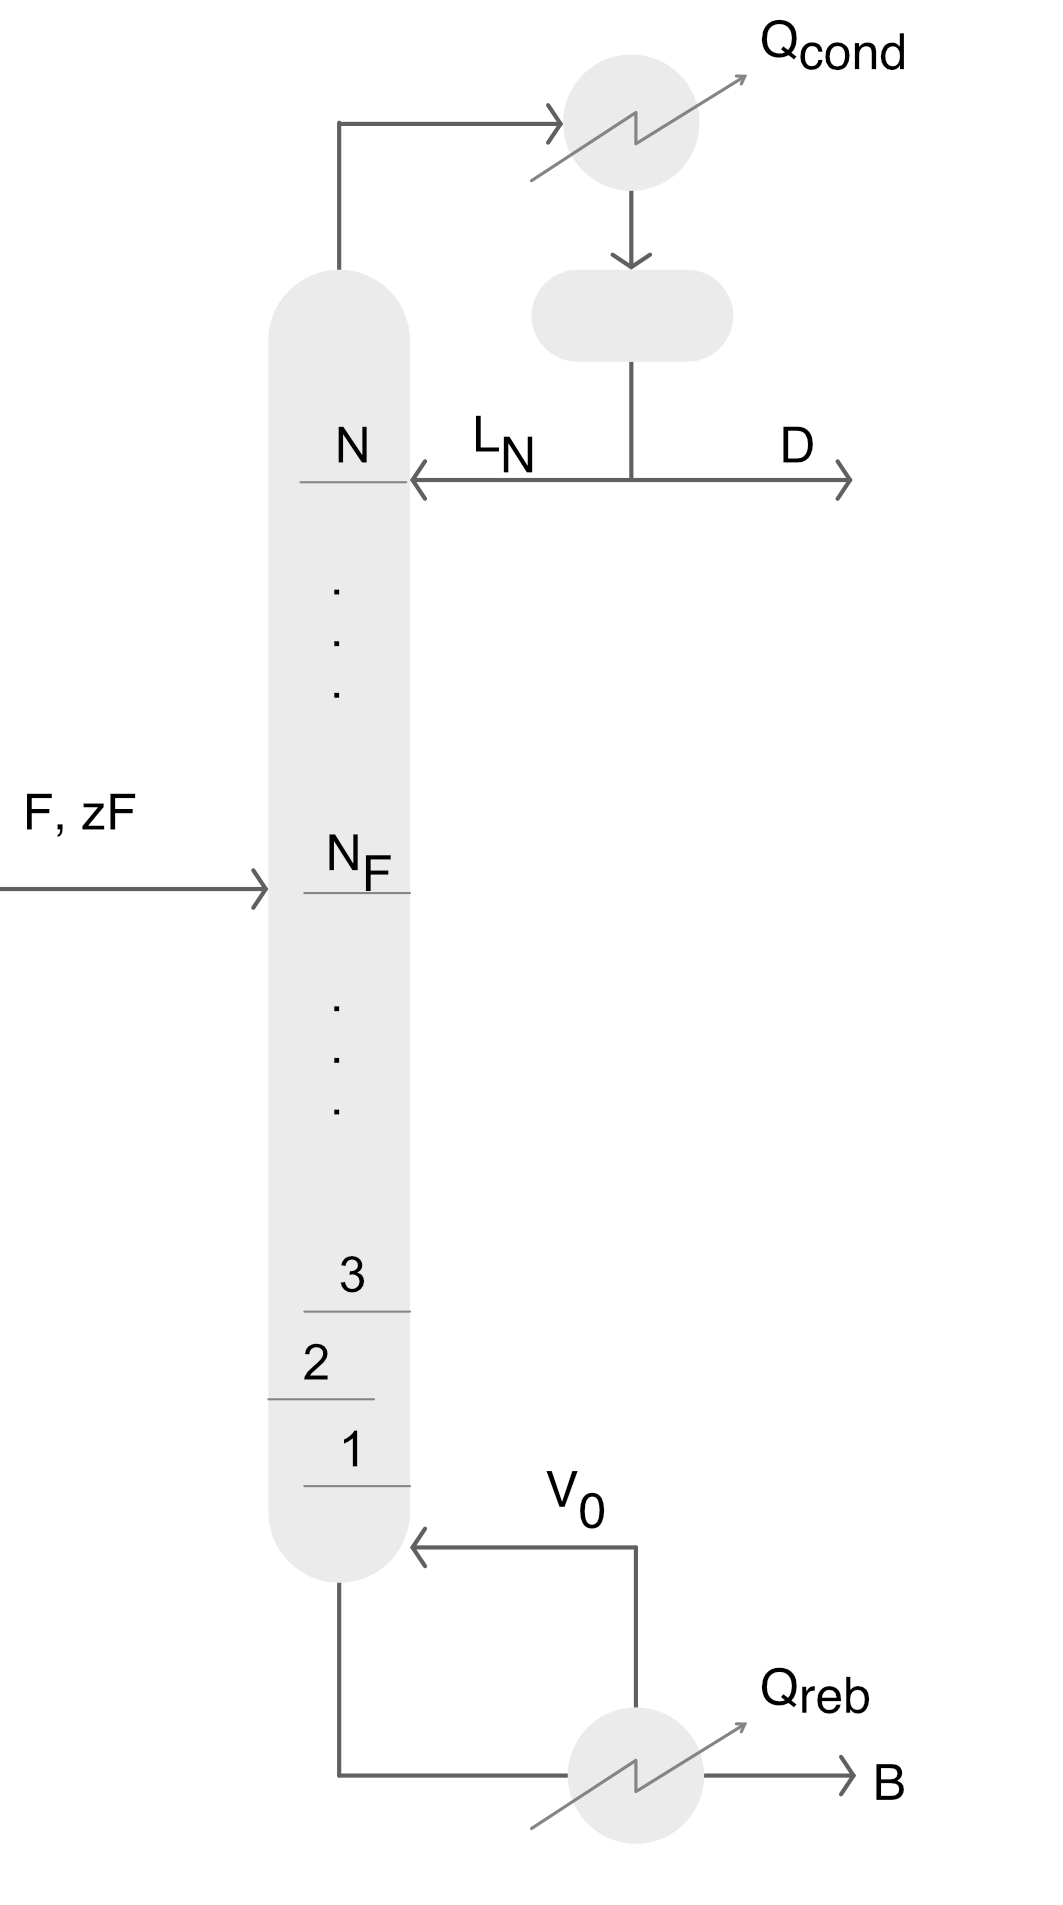
\includegraphics{gfx/Chapter06/basic_column.png}
    \caption{Depiction of a distillation column with $N$ trays, feed at stage $N_F$, and reboiler and condenser as stage 0 and $N+1$ respectively.}
    \label{fig:column}
\end{figure}



% The following are parameters of the model, determined by the experimental scenario or estimated via parameter estimation (see the next section).

% \begin{itemize}
%     \item$P_{top}$ is the pressure above stage $N$ in the column
%     \item$\Delta P_{strip}$ is the pressure drop in the stripping section (below feed stage)
%     \item$\Delta P_{rect}$ is the pressure drop in the rectifying section (feed stage and above)
%     \item$q_{N_F}$ is the vapor fraction in the feed
%     \item$z_{N_F}$ is the mol fraction in the feed
%     \item$F$ is the feed flowrate (kmol/hr)
%     \item$Q_{reb}$ is reboiler duty
%     \item$Q_{cond}$ is the condenser duty
%     \item$\alpha_{strip}$ is the Murphree efficiency in the stripping section (below feed stage)
%     \item$\alpha_{rect}$ is the Murphree efficiency in the rectifying section (feed stage and above)
% \end{itemize}

We assumed the pressure drop was constant throughout the simulation, which is reasonable given the experimental observations (a vacuum was used to keep pressure drop constant). Therefore the pressure on each stage is calculated using:

\begin{table}
    \centering
    \caption{Parameters of the distillation column model determined by experiments.}
    \begin{tabular}{cccc}
        \textbf{Parameter} & \textbf{Description} & \textbf{Scenario 1} & \textbf{Scenario 2}  \\
        \hline
         $P_{top}$ &  Pressure on stage N of the column &  0.5 & 0.22 \\ 
         $q_{N_F}$ & vapor fraction  in the feed & 1.0 & 1.0 \\
         $z_{N_F}$  & mole fraction of methanol in the feed &  0.5  & 0.5 \\
         $F$ & Feed flow rate &  333 mol/min  & 332 mol/min \\
    \end{tabular}
    \label{tab:parameters}
\end{table}

\begin{equation}
    P_i = P_{i+1} + \Delta P_i \;\; i=0\dots N
\end{equation}

where $\Delta P_i =\Delta P_{strip}$ for stages below feed stage and $\Delta P_i =\Delta P_{rect}$ for feed stage and above. The condenser pressure is calculated using $P_{cond}=P_{N} - \Delta P_{rect}$.

Constant parameters are shown in Table \ref{tab:parameters} and state variables in Table \ref{tab:state_variables}.
\begin{table}
    \centering
    \caption{State variables of the distillation column model.}
    \begin{tabular}{cc}
        \textbf{Variabe} & \textbf{Description}  \\
        \hline
         $x_i$ &  Liquid composition of methanol on stage $i$ \\
         $y_i$ & Vapor composition of water on stage $i$\\
         $L_i$ & Liquid flow on stage $i$  \\
         $V_i$  & Vapor flow on stage $i$ \\
         $T_i$  & Temperature on stage $i$ \\
         $T_i$  & Holdup on stage $i$ \\
    \end{tabular}
    
    \label{tab:state_variables}
\end{table}

\subsubsection{Material Balances}
Material balances are calculated for all stages including the reobiler and condenser.

\begin{equation}
\frac{dn_i}{dt} = L_{i+1}-L_i + V_{i-1}-V_i \; \forall i=1 \dots N_F-1, N_F+2 \dots N+1
\end{equation}

\begin{equation}
   \frac{dn_0}{dt} = L_1 - L_0 - V_0 
\end{equation}


\begin{equation}
    \frac{dn_{N+1}}{dt} = V_{N}-(L_{N+1} + D)    
\end{equation}

The  feed stage and the stage above the feed stage are treated separately:

\begin{equation}
    \frac{dn_{N_F}}{dt} = L_{N_F+1}-L_{N_F} + V_{N_F-1}-V_{N_F} + q_{N_F}F   
\end{equation}

\begin{equation}
   \frac{dn_{N_F+1}}{dt} = L_{N_F+2}-L_{N_F+1} + V_{N_F}-V_{N_F+1} + (1-q_{N_F})F 
\end{equation}


\subsubsection{Component Balances}

Component balances are calculated for all stages including the reobiler and condenser.

\begin{equation}
   \frac{d(x_{i} n_{i})}{dt}= y_{i-1}V_{i-1} -y_iV_i + x_{i+1}L_{i+1} - x_{i}L_i 
\end{equation}

\begin{equation}
    \frac{d(x_{N+1} n_{N+1})}{dt}  = y_NV_N - y_{N+1}V_{N+1} - x_{N+1}(L_{N+1} + D) 
\end{equation}


\begin{equation}
     \frac{d(x_{0} n_{0})}{dt} = L_1(x_1-x_0) + V_0(x_0-y_0) 
\end{equation}

The  feed stage and the stage above the feed stage are treated separately:

\begin{equation}
 \frac{d(x_{N_F} n_{N_F})}{dt}  = y_{N_F-1}V_{N_F-1} -y_{N_F}V_{N_F} + x_{N_F+1}L_{N_F+1} - x_{N_F}L_{N_F} + q_{N_F}z_FF   
\end{equation}

\begin{equation}
    \frac{d(x_{N_F+1} n_{N_F+1})}{dt} = y_{N_F+2}V_{N_F+2} -y_{N_F+1}V_{N_F+1} + x_{N_F}L_{N_F} - x_{N_F+1}L_{N_F+1} + (1-q_{N_F})z_FF 
\end{equation}


\subsubsection{Energy Balances}

For liquid enthalpy, we take a mole fraction weighted average of the specific enthalpies. Data is taken from Perry’s Chemical Engineering Handbook.

\begin{equation}
    h^{L,c}(T,P) = \int_{T_{ref}}^T C_p^c(\tau)d\tau 
\end{equation}

\begin{equation}
    h^L(T_i, P_i, x_i) = x_ih^{L,0}(T_i,P_i) + (1-x_i)h^{L,1}(T_i,P_i)
\end{equation}

\begin{equation}
    h^L_i := h^L(T_i, P_i,x_i)
\end{equation}

\begin{equation}
    h^L_{N_F} := h^L(T_{N_F}, P_{N_F},x_{N_F})
\end{equation}


For vapor enthalpy, we take a mole fraction weighted average of the specific enthalpies. Data is taken from Perry’s Chemical Engineering Handbook.

\begin{equation}
    h^{V,c}(T,P) = H^{vap, c}(T_{ref}) + 4R(T-T_{ref})
\end{equation}

\begin{equation}
    h^V(T_i, P_i, x_i) = x_i h^{V,0}(T_i,P_i) + (1-x_i) h^{V,1}(T_i,P_i)
\end{equation}


\begin{equation}
    h^V_i := h^V(T_i, P_i,x_i)
\end{equation}

\begin{equation}
    h^V_{N_F} := h^V(T_{N_F}, P_{N_F},x_{N_F})
\end{equation}

    
We assume that vapor holdup is negligible and therefore only consider the liquid holdup. Given these definitions, the enthalpy balances on the trays, reboiler and condenser are:

\begin{equation}
    \frac{d(n_ih^L_i)}{dt} =  h^L_{i+1}L_{i+1}-h^L_iL_i+h^V_{i-1}V_{i-1}-h^V_iV_i
\end{equation}

\begin{equation}
    \frac{d(n_0h^L_0)}{dt} = h^L_1L_1 - h^L_0L_0 - h^V_0V_0 + Q_{reb}
\end{equation}


\begin{equation}
    \frac{d(n_{N+1}h^L_{N+1})}{dt} = h^V_NV_{N}-h^L_{N+1}(L_{N+1} + D) + Q_{cond}
\end{equation}

Stage energy balance for all stages except the feed stage and  one above the feed stage:

\begin{equation}
    \frac{d(n_{N_F}h^L_{N_F})}{dt} = h^L_{N_F+1}L_{N_F+1}-h^L_{N_F}L_{N_F} + h^V_{N_F-1}V_{N_F-1}-h^V_{N_F}V_{N_F} + q_{N_F}F h^L_{N_F}
\end{equation}

where $q_{N_F}$ is the vapor fraction of the feed.

\begin{equation}
    \frac{d(n_{N_F+1}h^L_{N_F+1})}{dt} = h^L_{N_F+2}L_{N_F+2}-h^L_{N_F+1}L_{N_F+1} +h^V_{N_F} V_{N_F}-h^V_{N_F+1} V_{N_F+1} + (1-q_{N_F})Fh^V_{N_F}
\end{equation}


\subsubsection{Activity Coefficient Model}

We use the NRTL model for calculating the activity coefficients, though a variety of models could be used. The NRTL parameters for methanol-water are shown in Table X.

\begin{equation}
    \ln \gamma_{i,0} = x_2^2\biggl [\tau_{21} \biggl (\frac{G_{21}}{x_1+x_2G_{21}}\biggr)^2 + \frac{\tau_{12}G_{12}}{(x_2 + x_1 G_{12})^2} \biggr ]
\end{equation}

\begin{equation}
     \ln \gamma_{i,0} = x_1^2\biggl [\tau_{12} \biggl (\frac{G_{12}}{x_2+x_1G_{12}}\biggr)^2 + \frac{\tau_{21}G_{21}}{(x_1 + x_2 G_{21})^2} \biggr ]   
\end{equation}

\subsubsection{Pressure Balance}

Vapor pressure is calculated using Antoine’s equation with coefficients taken from NIST. 

\begin{equation}
    \log P_{i,k}^{sat} = A_k + \frac{B_k}{T_i + C_k}
\end{equation}

For trays ($i=1\dots N$), modified Raoult’s Law is used with Murphree efficiencies to account for deviations from equilibrium.

\begin{equation}
    y_i = \alpha_i\frac{x_i\gamma_i(T_i, P_i, x_i)P_0^{sat}(T_i)}{P} + (1-\alpha_i)y_{i-1}
\end{equation}

This leads to the bubble pressure balance:

\begin{equation}
    P = x_i\gamma_{i,0}(T_i, P_i, x_i)P^{sat}_{i,0} + (1-x_i)\gamma_{i,1}(T_i, P_i, (1-x_i))P^{sat}_{i,1}
\end{equation}

\subsubsection{Francis Weir Formula}

The Francis weir formula is used in dynamic mode to calculate liquid flow over the weir given a certain holdup. As shown in Figure \ref{fig:weir}, $h_i^{ow}$ from the the clear liquid to the weir. We can calculate this by taking the difference between the actual volume in the weir and a reference volume $n^v_{ref}$ (i.e., the volume if there was no crest) given the cross sectional area.

\begin{figure}
    \centering
    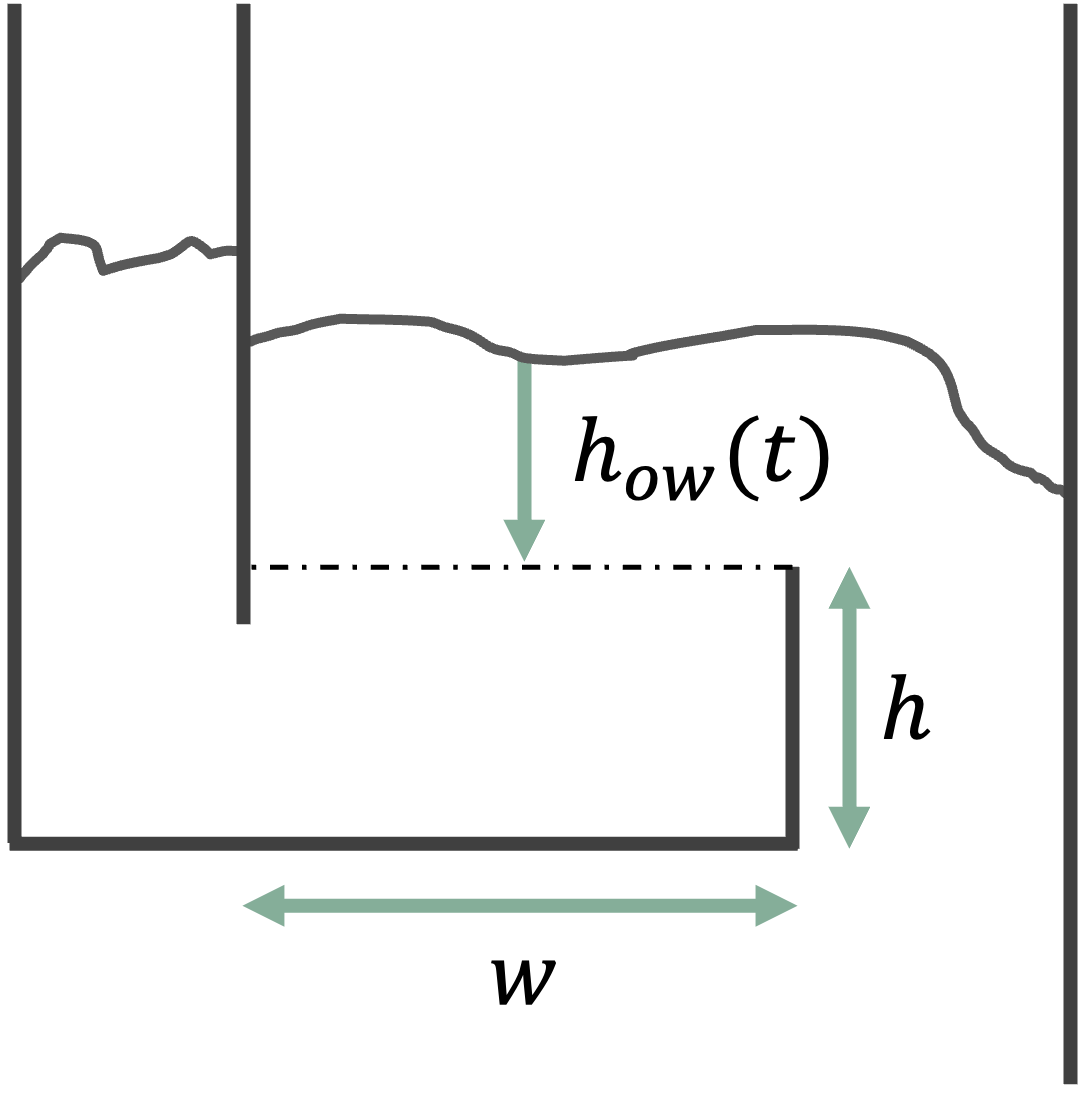
\includegraphics[width=0.4\textwidth]{gfx/Chapter06/weir.png}
    \caption{Diagram of weir showing $h_{ow}$ measured from the top of the clear liquid on a tray.}
    \label{fig:weir}
\end{figure}


\begin{equation}
    h^{ow}_i = \frac{n^v_i-n^v_{ref}}{A}
\end{equation}

The francis Weir formula for calculating flow over the Weir comes from the Bernoulli equation for the horizontal velocity $v$. We integrate from the top of the liquid (y=0) to the weir ($y=h_i^{ow}$)

\begin{equation}
    \frac{1}{2} \rho v^2 = \rho g y \ \Longrightarrow v(y) = \sqrt{2gy}
\end{equation}

\begin{equation}
    L_i^{vol} = \int_0^{h_i^{ow}} v(y)wdy = w\sqrt{2g}\int_0^{h_i^{ow}} y^{1/2}dy = \frac{2}{3}w\sqrt{2g}(h_i^{ow})^{3/2} 
\end{equation}


Substituting in above equation for  $h_i^{ow}$:

\begin{equation}
   L_i^{vol} = \frac{2}{3} w\sqrt{2g}\biggl(\frac{n^v_i-n^v_{ref}}{A}\biggr)^{3/2}  
\end{equation}

Diehl lumps all the constants into an estimatable parameter $W_{tray}$:

\begin{equation}
    L_i^{vol} = W_{tray}(n_i^v-n^v_{ref})^{3/2}
\end{equation}

\begin{equation}
    W_{tray} = \frac{2}{3}w\sqrt{2g}A^{-3/2}
\end{equation}

Based on measurements from BASF, we assume the diameter of the weir $w$ is 8 mm and the height of the weir $h$ is 10 mm. We take $h = 1\cdot10^{-2} m$ and $A=\pi w^2/4 = \pi(8 \cdot 10^{-3})^2/4 = 5.024 \cdot 10^{-5} m^2$, and g is the gravity of Earth. Therefore $W_{tray}^{init}=120149 \; m^{-3/2}s^{-1}$. $n^v_{ref}=Ah=1.45 \cdot 10^{-4} m$.t  We can use this initial estimate for $W_{tray}$ and then refine via dynamic parameter estimation.

Since the simulation is in molar flowrates, we need to convert from volumetric flowrates to molar flowrates:

\begin{equation}
    L_i = \rho(T_i, x_i)L^{vol}_i  
\end{equation}


where $\rho(T_i,x_i)$ is the volumetric density, calculated by a weighted average of the volumetric density of both components. Volumetric density come from Perry’s.

\begin{equation}
    \rho(T_i, x_i) = x_i\rho^0(T_i, x_i) + (1-x_i)\rho^1(T_i, x_i)
\end{equation}


\subsection{Parameter estimation to align simulations to experiments}

We created a simulation of a distillation column that can be aligned to experiments using a small amount of steady state data. The distillation simulation was built in Python using GEKKO \citep{Beal2018}, and the differential algebraic equation model used for the simulations is fully detailed in \ref{sec:distillation_model}. To align the simulation to experiments, a three step procedure, illustrated in Figure \ref{fig:simulation_workflow}, was followed: initialization, steady state solution with parameter estimation and dynamic simulation. All simulations were solved with the APOPT nonlinear programming solver to a tolerance $10^{-9}$ and relative tolerance $10^{-9}$.

\begin{figure}
    \centering
    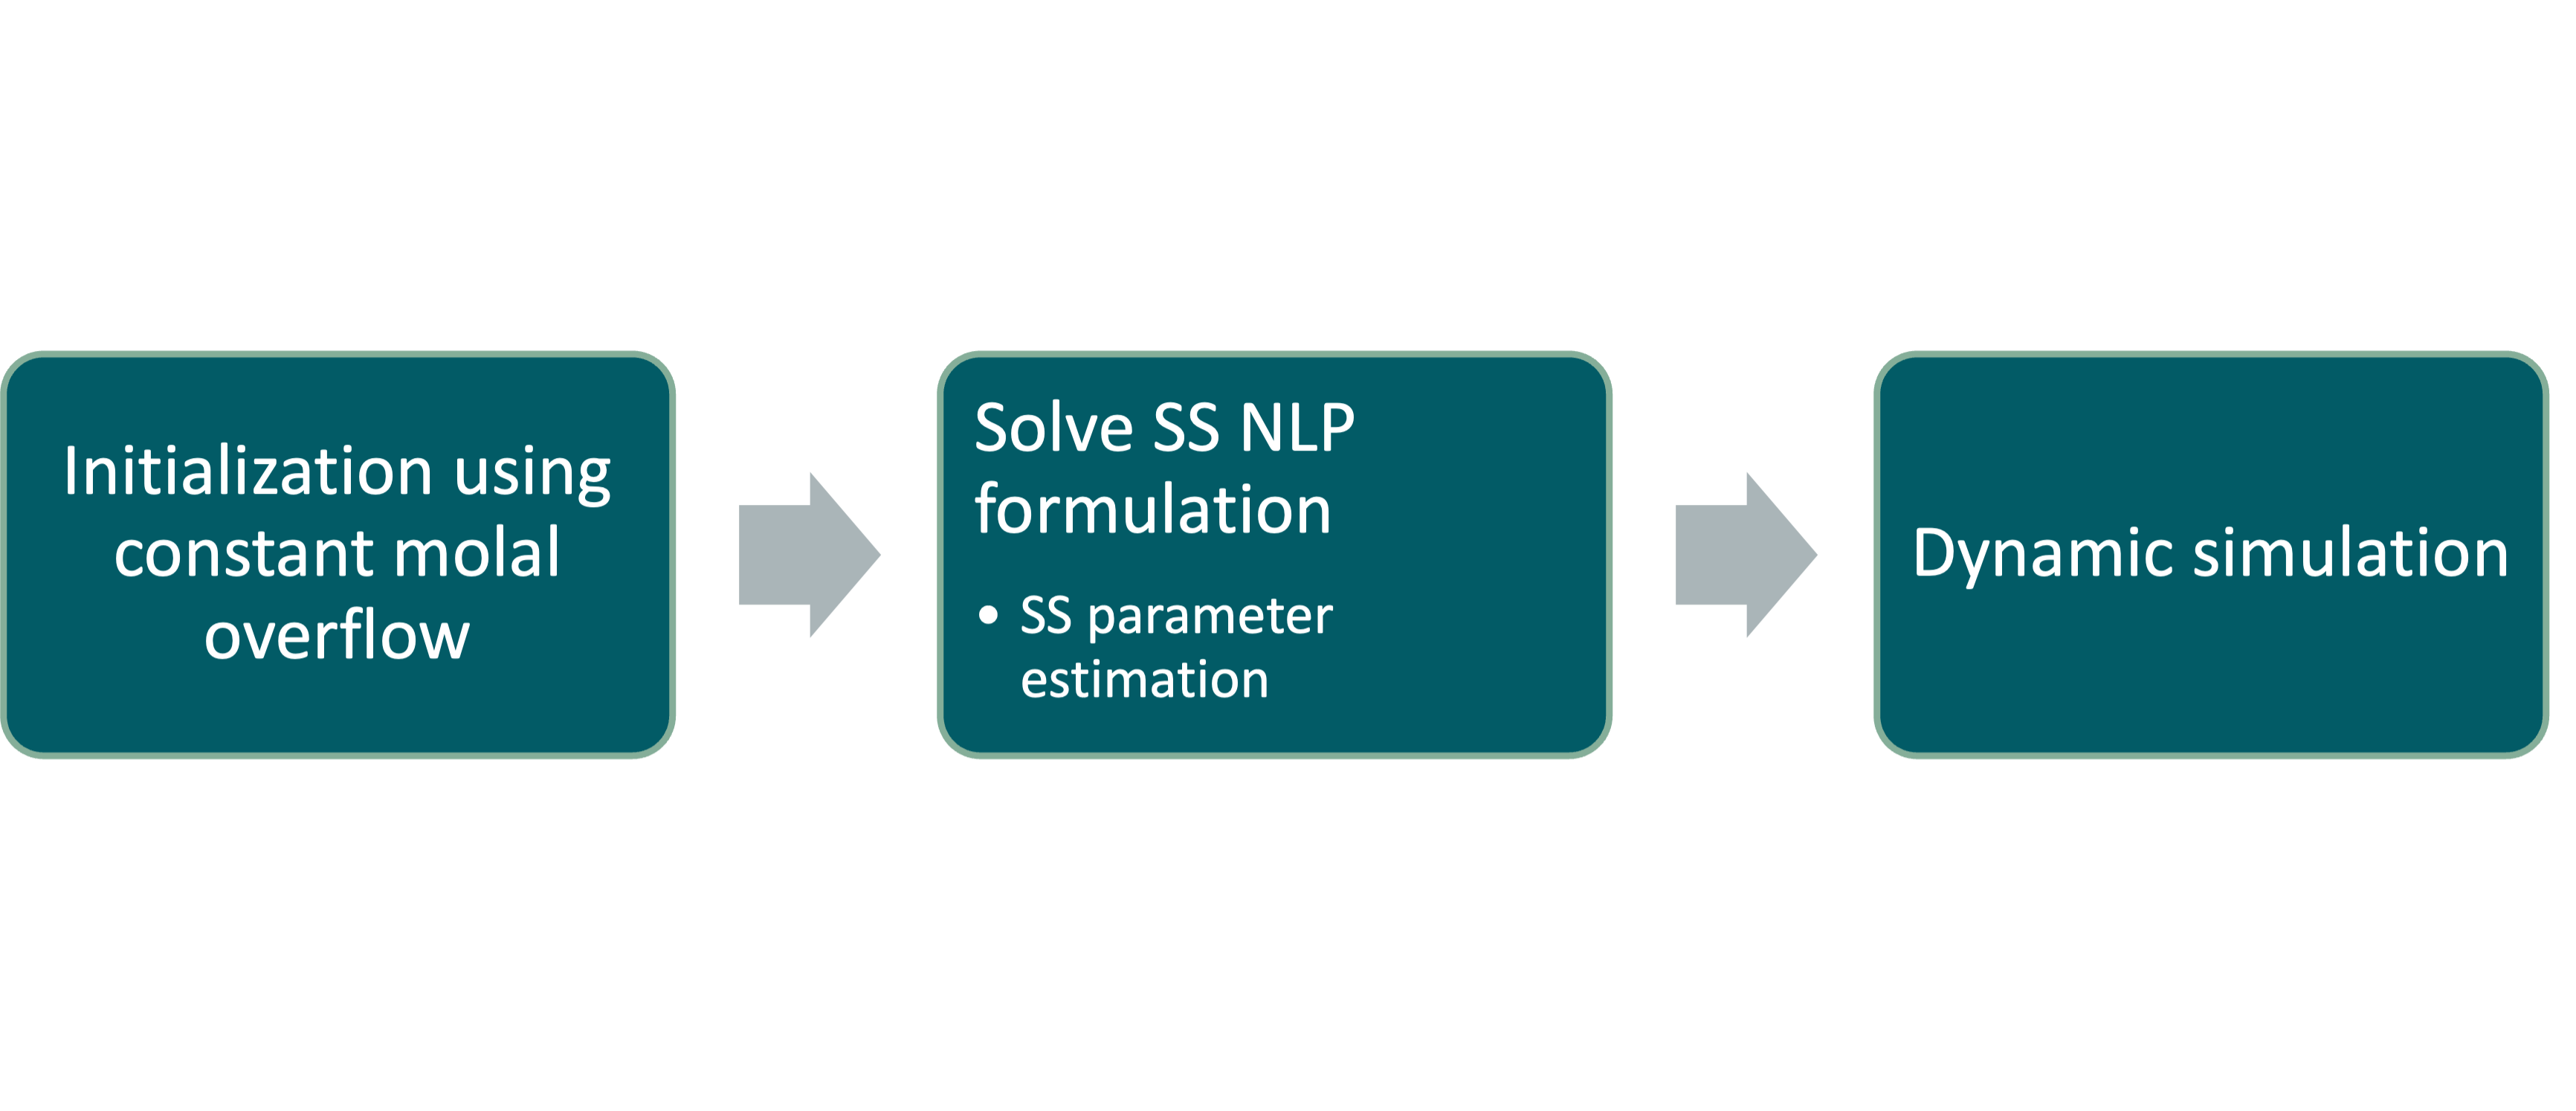
\includegraphics[width=\textwidth]{gfx/Chapter06/simulation_workflow.png}
    \caption{Schematic of the workflow for aligning the distillation simulation to experiments.}
    \label{fig:simulation_workflow}
\end{figure}

To initialize  the simulation, only the component material balances and pressure balances were solved. The constant molal overflow assumption was used, which states that there is constant liquid flow in the stripping and rectifying section respectively as well as constant vapor flow. 

Given the initialization, the full steady state simulation was then solved and used to generate the nominal values for steady state parameter estimation to the experimental data. The parameters estimated were the Murphree efficiencies and reboiler and condenser duties. While the condenser duty during dynamic simulation was fixed at the value from steady state parameter estimation, the reboiler duty was a manipulated variable; therefore, the steady-state estimated value of the reboiler duty served as an initial condition. The objective of the parameter estimation was to minimize the $L_1$ error between the simulation and experimental temperatures on stages 10, 22 and 35, as these stages were shown to be sensitive to changes in the parameters (see \ref{sec:sensitivity}). Therefore, the parameter estimation problem was formulated as:
%  The $l_1$ norm was chosen due to its improved  handling of outliers \citep{Safdarnejad2016}.
\begin{subequations}
    \begin{align}
        \min_{\boldsymbol \theta_{est}} \sum_{i\in \{10, 22, 35\}} \mathopen|T_i-T_i^{exp}\mathclose|\\
        s.t. \;\; 0 = \mathbf f(\mathbf X, \boldsymbol \theta)
    \end{align}
\end{subequations}
where $\mathbf X$ are the state variables in Table X  and $\boldsymbol \theta = \{\boldsymbol \theta_{est}, \boldsymbol \theta_{const} \}$.  $\boldsymbol \theta_{est}$ are the parameters to be estimated in Table \ref{tab:param_estimation} and $\boldsymbol \theta_{const}$ are the constant parameters in Table \ref{tab:parameters}. $\mathbf f$ is the system of equations represented by equations B.2-B.11, B.20-B.24, B.28-B.29, and B.36 with all derviatives set equal to zero. 
% \{\mathbf x, \mathbf y, \mathbf T, \mathbf L, \mathbf n\}$ 
\begin{table}[]
    \centering
    \begin{tabular}{cccc}
        \textbf{Parameter} & \textbf{Description} & \textbf{Initial Guess} & \textbf{Estimated Value}  \\
        \hline
         $\alpha_{strip}$ & Murphree efficiency in stripping section &  0.5 & 0.22 \\ 
         $\alpha_{rect}$ & Murphree efficiency in rectifying section & 0.5 & 1.0 \\
         % $\Delta P_{rect}$ & \thead{Pressure drop \\ in rectifying section} &  $\Delta P_{tot}/N$ \\ 
         % $\Delta P_{strip}$ & \thead{Pressure drop \\ in stripping section} &  $\Delta P_{tot}/N$ \\ 
         $ Q_{reb}$ & Reboiler duty at steady state &  0.245 kW  & 0.259 kW  \\
         $ Q_{cond}$ & Condenser duty at steady state &  -0.239 kW  & -0.253 kW
    \end{tabular}
    \caption{Parameters of the distillation column model estimated using experimental data. Estimates of the reboiler and condenser duties were made using the nominal values from the steady-state simulation, which in turn were guessed by plugging the flowrates and temperatures from the initialization into equations B.21 and B.22 with the derivatives set to 0.}
    \label{tab:param_estimation}
\end{table}

\begin{figure}
    \centering
    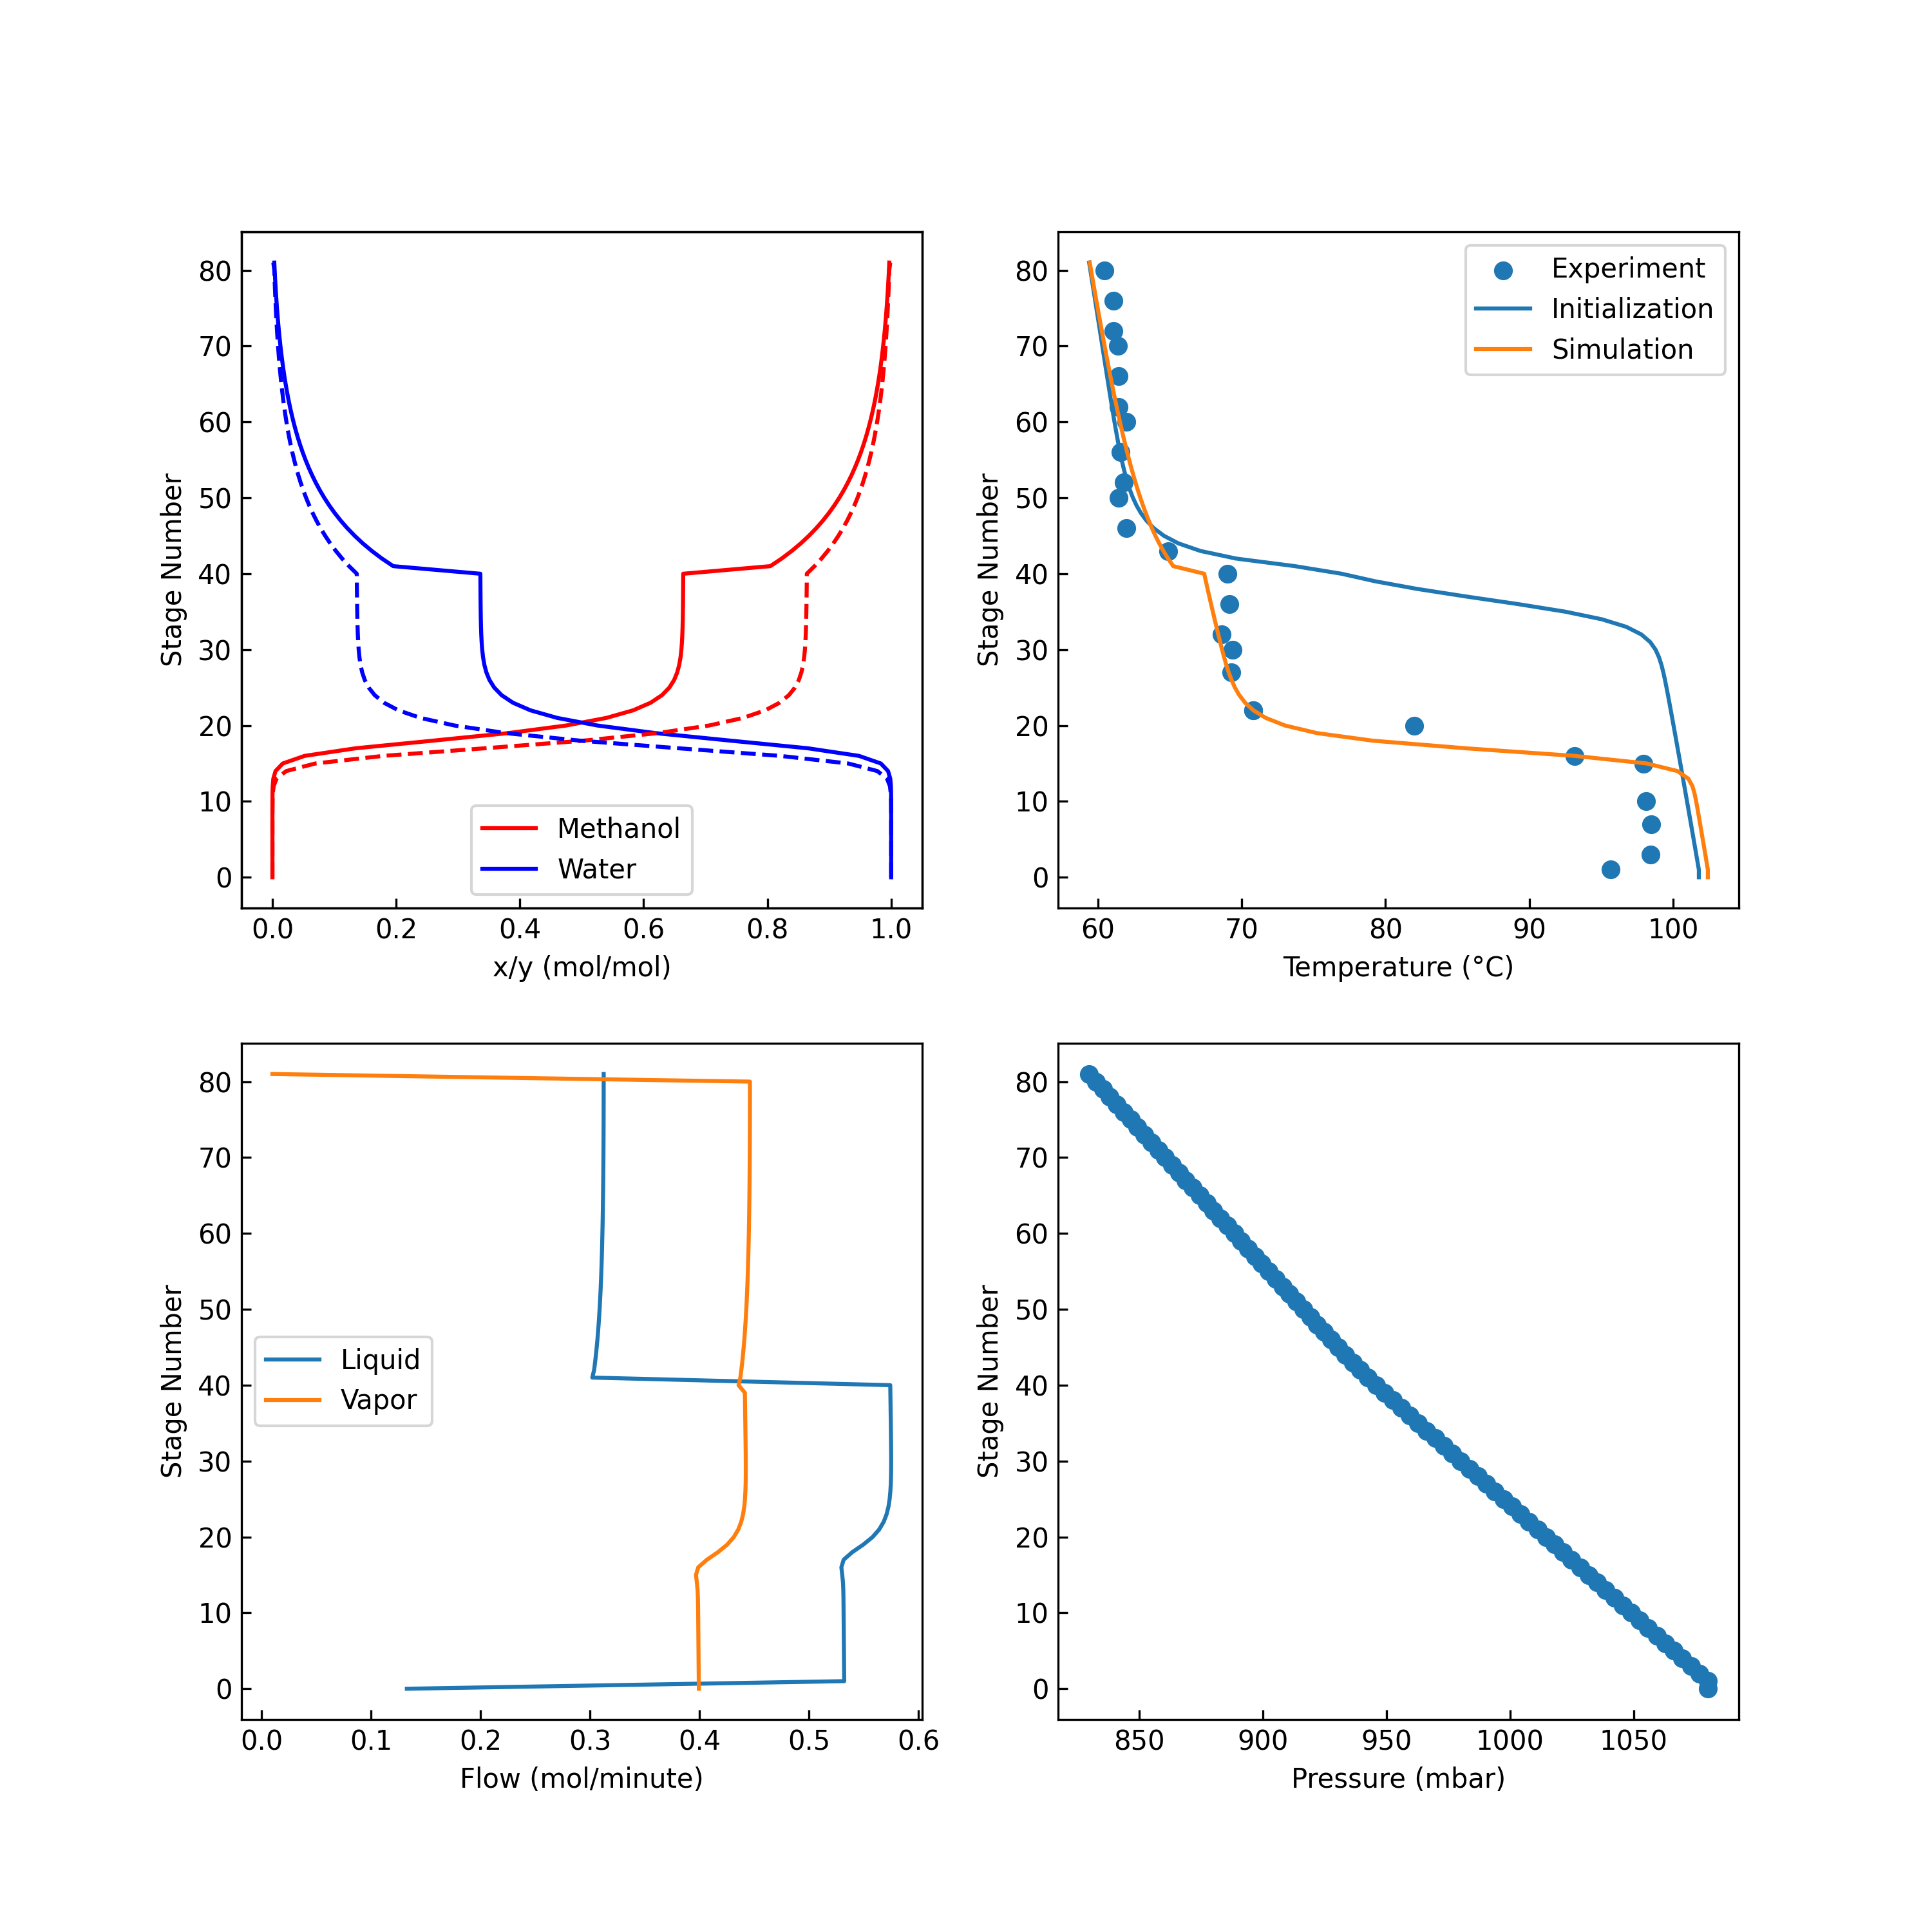
\includegraphics[width=\textwidth]{gfx/Chapter06/2021_11_17_steady_state_estimated.png}
    \caption{Steady state simulation after parameter estimation of a separation of 50/50 methanol-water separation in a distillation column with 80 bubble cap trays. \textbf{Top left}: Composition profile of the column with liquid composition in solid lines and vapor composition in dotted lines. \textbf{Top right}: Temperature profile of the simulation and experiments. \textbf{Bottom left}: Flow profile in column. \textbf{Bottom right}: Pressure profile in column.  }
    \label{fig:estimated}
\end{figure}

We used an average of the experimental stage temperatures over nine hours of steady state experimental data for parameter estimation. The resulting steady-state simulation after parameter estimation is shown in Figure \ref{fig:estimated}, which aligns well to the experimental temperature profile.  In Figure \ref{fig:validation}a, we show that using the estimated parameters with settings from a different day of experiments gives good alignment between simulation and experiment.  An example closed-loop dynamic simulation is shown in Figure Xb, which demonstrates that the dynamic simulation aligns closely to the experimental dynamics. 

% \begin{figure}
%     \begin{subfigure}[c]{0.49\textwidth}
%         \centering
%         \includegraphics[clip,width=\textwidth]{gfx/Chapter06/2021_11_18_steady_state_temperature.png}
%         \subcaption{}
%     \end{subfigure}
%     \begin{subfigure}[c]{0.49\textwidth}
%         \centering
%         \includegraphics[clip,width=\textwidth]{gfx/Chapter06/2021_11_18_steady_state_temperature.png}
%         \subcaption{}
%     \end{subfigure}
%     \caption{Caption}
%     \label{fig:validation}
% \end{figure}





\section{Results}

\section{Conclusion}